\chapter{Padding}\index{Padding}

Bei allen Algorithmen, die Nachrichten in festen Blöcken verarbeiten, muss die Nachrichtenlänge
ein Vielfaches der Blocklänge sein. Das gilt z.B. bei Blockciphern, aber auch bei Hashfunktionen etc. \\

\noindent Manchmal hilft Padding auch bei der Verschleierung des tatsächlichen Inhalts bei deterministischen Verfahren wie z.B. RSA oder klassische Cipher. \\

\noindent Deswegen versuchen wir, unsere Nachrichten in einer passenden Form aufzufüllen. Entweder weiß der Empfänger über das Padding Bescheid, oder er kann es - je nach konkreter 
Anwendung ignorieren. Es ist aber zu beachten, dass das Padding sich klar von der Nachricht untescheidet. Ein Negativbeispiel ist das Padding mit zufälligen Wörtern und 
Sätzen, wie bei der Geschichte aus dem zweiten Weltkrieg: \url{https://en.wikipedia.org/wiki/The_world_wonders}. \\

\noindent Es gilt zwar, dass ein Padding eine Nachricht immer verlängert, wir versuchen diese aber auf weniger als eine Blockgröße zu beschränken.

\section{Block cipher mode of operation}

Bei einem einfachen Padding, könnte der letzte Block mit einem regulären Bitmuster aufgefüllt werden:

\begin{itemize}
    \item nur 0er bzw. nur 1er
    \item abwechselnd 0 und 1
    \item so, dass der Empfänger das Padding entfernen kann
    \begin{itemize}
        \item z.B. lauter 0er und am Ende ein Byte, das angibt, wie viele Bytes entfernt werden sollen (z.B. \ldots, \verb|0x12, 0x15, 0x0, 0x0, 0x2|)
        \item dann muss aber jede Nachricht gepadded werden
        \item im schlimmsten Fall, muss ein gesamter Block angefügt werden
    \end{itemize}
\end{itemize}

Bei CBC gibt es folgendes Schema:

\begin{enumerate}
    \item Der letzte vollständige Block wird nochmals verschlüsselt
    \item Die linkesten $l$ Bit des neuen Ciphertext Blocks werden mit dem $l$-bit langen Klartextrest verxort
    \item Problem: Angreifer kann durch Manipulation des Ciphertextes gezielt Bits im letzten Klartextblock verändern
\end{enumerate}

\paragraph{Cipher Text stealing}\index{Cipher Text Stealing}

\begin{center}
    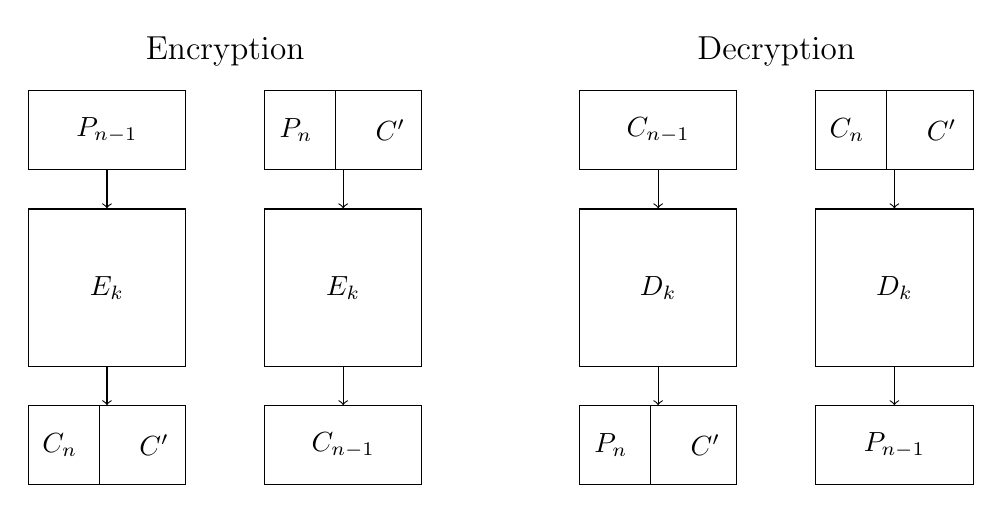
\begin{tikzpicture}[node distance=1cm and 1.5cm, every node/.style={align=center}]
      % Encryption Title
      \node (title1) [font=\large] at (-5,5) {Encryption};

      % Encryption - Left side
      \node (pn1) [draw, minimum width=2cm, minimum height=1cm] at (-6.5,4) {$P_{n-1}$};
      \node (ek1) [draw, minimum width=2cm, minimum height=2cm] at (-6.5, 2) {$E_k$};
      \node (cdash1) at (-5.9, 0) {$C'$};
      \node (cn1) at (-7.1, 0) {$C_n$};
      \node (auxc1) [draw, minimum width=2cm, minimum height=1cm] at (-6.5, 0) {};
      \draw (-6.6, 0.5) -- (-6.6, -0.5);
      \draw[->] (pn1) -- (ek1);
      \draw[->] (ek1) -- (auxc1);

      % Encryption - Right side
      \node (auxp1) [draw, minimum width=2cm, minimum height=1cm] at (-3.5, 4) {};
      \node (pn2) at (-4.1, 4) {$P_n$};
      \node (cdash2) at (-2.9, 4) {$C'$};
      \node (ek2) [draw, minimum width=2cm, minimum height=2cm] at (-3.5, 2) {$E_k$};
      \node (cn2) [draw, minimum width=2cm, minimum height=1cm] at (-3.5,0) {$C_{n-1}$};
      \draw (-3.6, 3.5) -- (-3.6, 4.5);
      \draw[->] (auxp1) -- (ek2);
      \draw[->] (ek2) -- (cn2);

      % Decryption Title
      \node (title2) [font=\large] at (2,5) {Decryption};

      % Decryption - Left side
      \node (cpn1) [draw, minimum width=2cm, minimum height=1cm] at (0.5,4) {$C_{n-1}$};
      \node (dek1) [draw, minimum width=2cm, minimum height=2cm] at (0.5, 2) {$D_k$};
      \node (dcdash1) at (1.1, 0) {$C'$};
      \node (dpn1) at (-0.1, 0) {$P_n$};
      \node (dauxc1) [draw, minimum width=2cm, minimum height=1cm] at (0.5, 0) {};
      \draw (0.4, 0.5) -- (0.4, -0.5);
      \draw[->] (cpn1) -- (dek1);
      \draw[->] (dek1) -- (dauxc1);

      % Decryption - Right side
      \node (dauxp1) [draw, minimum width=2cm, minimum height=1cm] at (3.5, 4) {};
      \node (dcn2) at (2.9, 4) {$C_n$};
      \node (dcdash2) at (4.1, 4) {$C'$};
      \node (dek2) [draw, minimum width=2cm, minimum height=2cm] at (3.5, 2) {$D_k$};
      \node (dpn2) [draw, minimum width=2cm, minimum height=1cm] at (3.5,0) {$P_{n-1}$};
      \draw (3.4, 3.5) -- (3.4, 4.5);
      \draw[->] (dauxp1) -- (dek2);
      \draw[->] (dek2) -- (dpn2);

    \end{tikzpicture}
\end{center}

Bei Cipher Text Stealing wird der vorletzte komplette Block $P_{n-1}$ verschlüsselt und in Teile $C_n$ und $C'$ aufgeteilt. 
Dann wird der letzte Block $P_n$ mit $C'$ gepadded und verschlüsselt. Dieser komplette Block $C_{n-1}$ kommt an die vorletzte Stelle des Ciphertexts und der noch nicht 
verwendete Teil $C_n$ wird angehängt. So kann die Nachricht mit Block Ciphern verschlüsselt werden, ohne sie zu verlängern.

\section{Hashfunktionen}\index{Padding!Hashfunktion}

\paragraph{MD5 und SHA-1} Hier muss die Nachricht um 64 Bits kleiner sein als ein Vielfaches von 512.
Das Padding ist eine 1 und entsprechend vielen 0 auf die benötigte Länge. Danach werden 64 Bit mit der Länge der ungepaddeten Nachricht angehängt, das erzeugt eine 
Nachricht mit einer durch 512 teilbaren Länge. \\

\noindent Diese Methode vermeidet, dass gleich beginnende und mit 0 endende Nachrichten denselben
Hashwert haben. Ohne das Einfügen der 1 vor dem Padding (und ohne angefügte Länge)
würden \verb|foo| und \verb|foo00| bzw. \verb|foo100| denselben Hash ergeben.

\section{Byteweise}

\paragraph{ANSI X.923} Mit 0x00 Bytes gepaddet, letztes Byte gibt Anzahl der Padding Bytes an

\paragraph{ISO 10126} Mit zufälligen Bytes gepaddet, letztes Byte gibt Anzahl der Padding Bytes
an (mittlerweile zurückgezogen)

\paragraph{ISO 7816} (ISO 9797) Ein fixes Byte markiert Beginn des
Paddings, danach mit 0x00 aufgefüllt. Im Wesentlichen bei Smartcards
verwendet.

\paragraph{PKCS5/7} (RFC3852) Letzter Block gepaddet mit $n$ Bytes, alle mit Wert $n$. Mögliche Varianten sind also
\begin{itemize}
    \item \verb|0x01|
    \item \verb|0x02 0x02|
    \item \verb|0x03 0x03 0x03|
    \item \ldots
\end{itemize}

\paragraph{Zero Padding} Mit 0x00 aufgefüllt, ist nicht reversibel

\section{RSA}\index{Padding!RSA}

Zu kurze Nachrichten problematisch zu verschlüsseln. Ursprünglich wurde einfach mit Zufallsdaten auf bestimmte Länge aufgefüllt
Im ersten Public-Key Cryptography Standards (PKCS) < v2.0:
\begin{itemize}
    \item v1.5 = RFC 2313
    \item EM = 0x00||BT||PS||0x00||M
    \item BT (Block Type) ist
    \begin{itemize}
        \item 0x00 oder 0x01 für Private Key Operationen (signieren)
        \item 0x02 für Public Key Operationen (verschlüsseln)
    \end{itemize}
    \item PS (Padding String) ist ($k$ - Länge von $M$ - 3) Bytes lang, mindestens aber 8
    \begin{itemize}
        \item k = Länge des Modulus in Byte
        \item PS ist 0x00 für BT = 0x00, 0xFF für BT = 0x01 und zufällig für BT = 0x02
    \end{itemize}
    \item Problem: nicht übermäßig zufällig, Struktur der Klartextnachricht erratbar
    \item Bleichenbacher Angriff (\url{https://web.archive.org/web/20120204040056/}, \url{http://www.bell-labs.com/user/bleichen/papers/pkcs.ps})
\end{itemize}

Mittlerweile iwrd üblicherweise Optimal Asymmetric Encryption Padding (OAEP) verwendet, eingeführt in PKCS\#1 v2.0

\section{OAEP (Optimal Asymmetric Encryption Padding)}\index{OAEP}\index{Optimal Asymmetric Encryption Padding}\index{Padding!OAEP}

\paragraph{Ablauf}

Sei $M$ eine Nachricht der Länge $m$ und $h$ die Länge des Hashes.

\begin{enumerate}
    \item Label $L$ wird gehasht, Ergebnis ist $l_{Hash}$
    \item Padding String $p$ aus 0x00 wird an $l_{Hash}$ angehängt, sodass die resultierende Länge um ($m + h + 2$) Bytes kürzer ist als der RSA Modulus in Bytes ($k$)
    \item es wird 0x01 und $M$ an den Block angehängt, daraus resultiert Data Block (DB), der um $h+1$ Bytes kürzer ist als $k$
    \begin{itemize}
        \item DB = $l_{Hash}$ || $p$ || 0x01 || $M$
    \end{itemize}
    \item Ein zufälliger String $r$ (ein sog. seed) mit Länge $h$ wird erzeugt
    \item $r$ wird mittels der Mask Generation Function (MGF) auf die Länge $(k - h - 1)$ Bytes vergrößert und mit DB verxort, das Ergebnis ist $DB_{masked}$
    \item $DB_{masked}$ wird mittels MGF auf die Länge $h$ verkleinert und mit $r$ verxort, das Ergebnis ist $r_{masked}$
    \item Encoded Message (EM) entsteht durch Konkatenation von 0x00, $r_{masked}$ und $DB_{masked}$
    \begin{itemize}
        \item EM = 0x00 || $r_{masked}$ || $DB_{masked}$
        \item Das erste 0 Byte dient dazu, zu garantieren, dass EM tatsächlich kleiner ist als der Modulus $n$: beide haben $k$ Byte, aber da in EM das höchstwertige Byte 
        0 ist, gilt sicher immer: EM $< n$.
    \end{itemize}
    \item EM wird mittels RSA verschlüsselt, d.h. $C = \text{EM}^e \mod n$
\end{enumerate}

\begin{figure}[h]
    \includegraphics[width=0.4\textwidth]{figures/fig08-oaep}
    \centering
    \caption{Ablauf OAEP Verschlüsselung}
\end{figure}

\paragraph{Entschlüsselung}

\begin{enumerate}
    \item Empfänger bekommt Ciphertext $C$ und Label $L$
    \item Generiert EM aus $C$ mittels seines privaten Schlüssels, dabei muss das erste Byte von EM 0x00 sein
    \item Die nächsten $h$-Bytes sind $r_{masked}$, der Rest ($k - h - 1$) ist $DB_{masked}$
    \item $DB_{masked}$ wird mittels MGF auf Länge $h$ gebracht und mit $r_{masked}$ verxort, resultiert im Seed $r$
    \item $r$ wird mittels MGF auf Länge von $DB_{masked}$ gebracht und damit verxort, ergibt $DB$
    \item $DB$ muss beginnen mit dem Hash von $L$ (bzw. Hash des leeren Strings in PKCS\#1), gefolgt von beliebig vielen 0x00 und einer 0x01
    \item Nach 0x01 steht die Nachricht $M$
\end{enumerate}

Sowohl $DB_{masked}$ als auch $r_{masked}$ müssen vollständig bekannt sein, um $M$ zu rekonstruieren zu können. Mittels $DB_{masked}$ kann $r$ rekonstruiert werden, 
mittels $r$ dann $DB$ und in Folge $M$.
OAEP erschwert die Rekonstruktion des Klartextes für einen Angreifer. \\

\noindent Die in PKCS\#1 empfohlene Parameter für RSAES-OAEP (RSA Encryption Standard OAEP) sind 
\begin{itemize}
    \item Hash: SHA-1/256/384/512, d.h. die Hashlänge ist 20, 32, 48 oder 64 Bytes
    \item Mask Generation Function: MGF1
    \begin{itemize}
        \item $k$ Runden, in jeder Runde werden $h$ Bytes zum Output hinzugefügt, bis die gewünschte Länge erreicht ist
        \item In jeder Runde:
        \begin{itemize}
            \item 32-bit Zähler wird inkrementiert
            \item Initialwert wird mit aktuellem Zähler konkateniert und gehasht
            \item Ergebnis wird an Endergebnis angehängt
        \end{itemize}
    \end{itemize}
\end{itemize}
